% A字 引入：△ABC，DE∥BC, 证 △ADE~△ABC
\documentclass[tikz,border=4pt]{standalone}
\usepackage{ctex}
\usepackage{amsmath}
\usetikzlibrary{calc}
\begin{document}
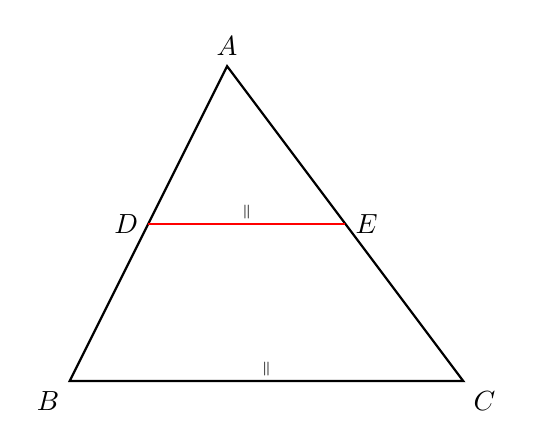
\begin{tikzpicture}[scale=1.0, thick]
  \coordinate (A) at (2,4);
  \coordinate (B) at (0,0);
  \coordinate (C) at (5,0);
  \coordinate (D) at ($(A)!0.5!(B)$);
  \coordinate (E) at ($(A)!0.5!(C)$);
  \draw (A)--(B)--(C)--cycle;
  \draw[red] (D)--(E);
  % 平行标记
  \node at ($(D)!0.5!(E)+(0,0.15)$) {\tiny $\parallel$};
  \node at ($(B)!0.5!(C)+(0,0.15)$) {\tiny $\parallel$};
  \node[above] at (A) {$A$};
  \node[below left] at (B) {$B$};
  \node[below right] at (C) {$C$};
  \node[left] at (D) {$D$};
  \node[right] at (E) {$E$};
\end{tikzpicture}
\end{document}
